\chapter{mAyAcwkada itihAsa matutx racane}

itihAsavanunx noVDidAga BArata, ciVnA, arabf matutx pAshAcxtayx rASaTxrXgaLalilx pArxciVna kAladalelxV mAyAcwkagaLu baLakeyalilxtutx eMdu gotAtxgutatxde.

mAyAcwkagaLu kirxsatx pUvaRdalelxV hiMdU deVshadalilx AraMBavAyitu. idanunx kAnfsATxMTinoVpalina mAsokxVpalasf eMbuvanu ivugaLanunx kalitu yUroVpiyananxrige heVLikoTaTx eMdu tiLidubaMdide. kirx.~sha. {\rm 1-2} neV shatamAnada nAgAjuRna, kirx.~sha. {\rm 505} ralilx varAhamihiVra mAyAcwkada bagegx ulelxVKisidAdxre. nArAyaNa paMDitaniMda racitavAda ``gaNita kwmudi (kirx.~sha. {\rm 1356})" eMba garxMthada parxkAra mAyAcwkagaLa adhayxyana hiMdU deVshadalilx unanxta maTaTxdalilxtutx eMdu gotAtxgutatxde.

mahArASaTxrX rAjayxda nAsikf eMba deVvAlayada goVDeyalilx oMdu mAyAcwka kaMDubaMdide ideV nAsikf mAyAcwka. BAratada jeYna gaNitajacnxrigU mAyAcwkada bagegx visheVSavAda jAcnxnavitutx eMdu tiLidubaMdide. eraDu riVtiya avara mAyAcwkagaLanunx noVDabahudu. KajurAhoVnalilx pAshavxRnAtha deVvAlayadalilx $4\times 4$ karxmada oMdu mAyAcwka ketitxruvudu kaMDubaMdide.

mAnadeVvasUri eMbuvanu tananx `laGushAMti sotxVtarxdalilx' {\rm 16} manegaLa mAyAcwkada racane bagegx hAgU adanunx biVjamaMtarxvAgi baLasuvudanunx tiLisi\-dAdxne.

shuBasuMdara eMbuvanu tananx yugAdi deVvasotxVtarxdalilx {\rm 25} manegaLa matutx {\rm 64} manegaLa mAyAcwka niVDidAdxne.

dhamARnaMdaneMbuvanu {\rm 64} manegaLa mAyAcwka racisuva bagegx tiLisidAdxne. idariMda BAratadalilx mAyAcwkagaLa adhayxyana bahaLa hiMdiniMda tiLiditutx eMdu gotAtxgutatxde.

mAyAcwkagaLanunx rakASxyaMtarx matutx tAyitagaLalilx ketitxsi toVLigoV, kutitxgegoV dharisutitxdadxraMte.

Adare oMdu AshacxyaRkara saMgati eMdare AyaRBaTa, barxhamxgupatx, mahAviVrA\-cAyaR matutx eraDaneV BAsakxrAcAyaRru I mAyAcwkada bagegx parxsAtxpamADilalx.

Adhunika hesarAMta BAratada gaNitajacnx shirxVnivAsa rAmAnujanf pwrxDhashAleyalilx\-dAdxginiMda mAyAcwkada bagegx kaqSimADidAdxre. avara modala eraDu TipapxNi pusatxka\-gaLalilx mAyAcwkada racane bagegx adaralUlx $3\times 3$ dajeRya mAyAcwkada bagegx tiLisidAdxre.

rAmAnujanfravaralalxde inUnx modalAdavaru, mAyAcwkada bagegx adhayxyana mADi aDaDxsAlu, kaMbasAlu, kaNaRsAlu motatx sonenx Agiruva shUnayx mAyAcwka\-gaLa sahAyadiMda biVjagaNitada nitayx samateyanunx biDisabahudu eMdidAdxre.

puNeya BAratiVya ``saMKAyxmAMtirxka'' reMdeV hesaruvAsiyAda Di.~Arf. kaperxVkarfravarU mAyAcwkada bagegx keY ADisidAdxre.

{\rm 18} neya shatamAnadalilx meYsUrina mahArAjarAgidadx mumumxDi kaqSaNxrAja oDeyarf tamamx `caturaMga sAra savaRsavx' eMbudaralilx saMKeyxgaLanunx caduraMgada kudure, naDigeyalilx Ane naDigeyalilx, rAjana naDigeyalilx iruvaMte aneVka bageya $8\times 8$ matutx $12\times 12$ ra sherxVNiya cwkagaLanunx racisuvudanunx tiLisidAdxre.

aMtU mAyAcwkavanunx kelavaru dhAmiRka cihenxyAgi mUDanaMbike iruvavaru deVhakekx BUta perxVtagaLiMda rakaSxNe hAgU roVganivAraka asatxrXvAgi, yaMtarx, maMtarx, taMtarx matutx mAyAmATa muMtAdavugaLalilx, gaNitajacnxru saMKAyxloVkada adhayxyanakekx matutx kelavu yuva piVLige manaraMjanegAgi mAyAcwkagaLanunx upayoVgisutitxruvudu kaMDubaMdide.

hiVge elAlx riVtiya janarigU mAyAcwka oMdu sAvxrasayxkaravAda viSaya\-vAgide.

{\bf mAyAcwka eMdareVnu?}

oMdu doDaDx cwkadalilxruva, saNaNx saNaNx samAna cwkagaLalilx gotAtxda karxmadiMda saMKeyxgaLiMda tuMbiruva (kaDeVpakaSx {\rm 9}) aDaDxsAlu, kaMbasAlu matutx mUleyiMda mUlege (kaNaRsAlu) iruva saMKeyxgaLanunx kUDidAga yAvAgalU motatx samanAgidadxre A cwkavanunx mAyAcwka enunxtetxVve.

A motatxvanunx mAyA motatx athavA mAyAsaMKeyx enunxtetxVve.

mAyAcwkagaLanunx racisuvudu heVge? eMbudanunx kaDeyalilx oMderaDu udAharaNe mUlaka I leVKanadalilx tiLiside. AdarU idoMdu mAyAcwkagaLa bagegx oMdu pakiSxnoVTa.

halavaru mAyAcwkagaLa bagegx vivaravAgi pusatxkavanunx baredidAdxre. avaralilx\break DA|| esf. bAlacaMdarxrAvf ``mAyAcwkagaLa sAvxrasayx'', shirxV~bi.~ke. vishavxnAtharAvf ``mAyAcwkagaLa mAyA parxpaMca'' muKayxvAdavugaLu.

\begin{center}
\begin{tabular}{|>{$}c<{$}|>{$}c<{$}|>{$}c<{$}|}
\hline
8 & 1 &6\\
\hline
3 & 5 &7\\
\hline
4 & 9 &2\\
\hline
\end{tabular}
\end{center}

meVle barediruva oMdu doDaDx cwkadalilx, saNaNx {\rm 9} cwkagaLive. aDaDxsAlinalilx {\rm 3} manegaLive, kaMbasAlinalilx {\rm 3} manegaLive. AdadxriMda idu {\rm 3} neya sherxVNi (dajeR)ya mAyAcwka aMdare $(2n+1)$ rUpada besasaMKeyx sherxVNi (dajeR) mAyAcwka. yAvudeV aDaDxsAlina, kaMbasAlina, mUleyiMda mUlege (kaNaRsAlu) ivugaLalilxna saMKeyxgaLa motatx {\rm 15}. {\rm 1} riMda {\rm 9} ra tanaka saMKeyxgaLanunx oMdoMdeV sala baredide.
\begin{alignat*}{3}
\text{aDaDxsAlu }\qquad  && 8+1+6&&=15\\[0.2cm]
&&3+5+7&&=15\\
&&4+9+2&&=15\\
\text{kaMbasAlu}\qquad  &&8+3+4&&=15\\
&&1+5+9&&=15\\
&&6+7+2&&=15\\[0.2cm]
\text{mUleyiMda mUlege} \qquad & & 4+5+6&&=15\\[-0.2cm]
\text{kaNaRsAlu} \qquad  &&\\[-0.5cm]
&&8+5+2&&=15
\end{alignat*}

mAyAcwkadalilx iSeTxV saMKeyx aMkaNagaLirabeVkeMdilalx, pArxraMBika saMKeyx ideV AgirabeVkeMdilalx, yAva saMKeyxyiMdalAdarU pArxraMBisabahudu. namage beVkAda motatxvu laBisuvaMte mAyAcwka racisabahudu. mAyAcwkagaLa racaneyalilx\break baLasuva saMKeyxgaLu aMkagaNita sherxVDhiyalilxrutatxve. udA:  $1, 2, 3, 4,\ldots\ldots\break  5, 10, 15, 20,\ldots  4, 7, 10, 13\ldots\ldots$ itAyxdi.
 
meVle barediruva mAyAcwkavanenxV beVre riVtiyalilx aMdare {\rm 7} riVtiyalilx baredide.

\begin{center}
\begin{minipage}[p]{2cm}
\begin{tabular}{|>{$}c<{$}|>{$}c<{$}|>{$}c<{$}|}
\hline
6 & 1 & 8\\
\hline
7 & 5 & 3\\
\hline
2 & 9 & 4\\
\hline
\end{tabular}
\end{minipage}
\quad
\begin{minipage}[l]{2cm}
\begin{tabular}{|>{$}c<{$}|>{$}c<{$}|>{$}c<{$}|}
\hline
8 & 3 & 4\\
\hline
1 & 5 & 9\\
\hline
6 & 7 & 2\\
\hline
\end{tabular}
\end{minipage}
\quad
\begin{minipage}[p]{2cm}
\begin{tabular}{|>{$}c<{$}|>{$}c<{$}|>{$}c<{$}|}
\hline
6 & 7 & 2\\
\hline
1 & 5 & 9\\
\hline
8 & 3 & 4\\
\hline
\end{tabular}
\end{minipage}
\end{center}

\begin{center}
\begin{minipage}[l]{2cm}
\begin{tabular}{|>{$}c<{$}|>{$}c<{$}|>{$}c<{$}|}
\hline
4 & 9 & 2\\
\hline
3 & 5 & 7\\
\hline
8 & 1 & 6\\
\hline
\end{tabular}
\end{minipage}
\quad
\begin{minipage}[p]{2cm}
\begin{tabular}{|>{$}c<{$}|>{$}c<{$}|>{$}c<{$}|}
\hline
2 & 9 & 4\\
\hline
7 & 5 & 3\\
\hline
6 & 1 & 8\\
\hline
\end{tabular}
\end{minipage}
\quad
\begin{minipage}[l]{2cm}
\begin{tabular}{|>{$}c<{$}|>{$}c<{$}|>{$}c<{$}|}
\hline
4 & 3 & 8\\
\hline
9 & 5 & 1\\
\hline
2 & 7 & 6\\
\hline
\end{tabular}
\end{minipage}
\quad
\begin{minipage}[l]{2cm}
\begin{tabular}{|>{$}c<{$}|>{$}c<{$}|>{$}c<{$}|}
\hline
2 & 7 & 6\\
\hline
9 & 5 & 1\\
\hline
4 & 3 & 8\\
\hline
\end{tabular}
\end{minipage}
\end{center}

alilxge oTuTx {\rm 8} vividha riVtiyalilx mAyAcwkagaLanunx racisidaMtAyitu. inunx mADalu sAdhayxvilalx beVkAdare parxyatinxsi.

aDaDxsAlina motatx {\rm 15}, kaMbasAlina motatx {\rm 15}, mUleyiMda mUlege (kaNaRsAlu) motatx {\rm 15.} oMdariMda AraMBisi oMBatatxra tanaka saMKeyxgaLanunx oMdoMdeV sala baredide.

mAyAcwkavanunx AgaleV heVLidaMte oMdariMdaleV AraMBisabeVkeMdilalx. Iga noVDi {\rm 0} yiMda AraMBisi {\rm 8}ra tanaka karxmavAgi {\rm 9} saMKeyxgaLanunx upayoVgisi mAyAcwka raciside.

aDaDxsAlina, kaMbasAlina mUleyiMda mUlege (kaNaRsAlu) motatx {\rm 12}. {\rm 12} mAyA motatx athavA mAyAsaMKeyx, idU saha $(2n+1)$ rUpada besasaMKeyx sherxVNi (dajeR) mAyAcwka

\begin{center}
\begin{minipage}[l]{2cm}
\begin{tabular}{|>{$}c<{$}|>{$}c<{$}|>{$}c<{$}|}
\hline
7 & 0 & 5\\
\hline
2 & 4 & 6\\
\hline
3 & 8 & 1\\
\hline
\end{tabular}
\end{minipage}
\quad
\begin{minipage}[p]{2cm}
\begin{tabular}{|>{$}c<{$}|>{$}c<{$}|>{$}c<{$}|}
\hline
5 & 6 & 1\\
\hline
0 & 4 & 8\\
\hline
7 & 2 & 3\\
\hline
\end{tabular}
\end{minipage}
\quad
\begin{minipage}[l]{2cm}
\begin{tabular}{|>{$}c<{$}|>{$}c<{$}|>{$}c<{$}|}
\hline
5 & 0 & 7\\
\hline
6 & 4 & 2\\
\hline
1 & 8 & 3\\
\hline
\end{tabular}
\end{minipage}
\quad
\begin{minipage}[l]{2cm}
\begin{tabular}{|>{$}c<{$}|>{$}c<{$}|>{$}c<{$}|}
\hline
7 & 2 & 3\\
\hline
0 & 4 & 8\\
\hline
5 & 6 & 1\\
\hline
\end{tabular}
\end{minipage}\\ 
\end{center}

\begin{center}
\begin{minipage}[l]{2cm}
\begin{tabular}{|>{$}c<{$}|>{$}c<{$}|>{$}c<{$}|}
\hline
1 & 8 & 3 \\
\hline
6 & 4 & 2\\
\hline
5 & 0 & 7\\
\hline
\end{tabular}
\end{minipage}
\quad
\begin{minipage}[p]{2cm}
\begin{tabular}{|>{$}c<{$}|>{$}c<{$}|>{$}c<{$}|}
\hline
1 & 6 & 5\\
\hline
8 & 4 & 0\\
\hline
3 & 2 & 7\\
\hline
\end{tabular}
\end{minipage}
\quad
\begin{minipage}[l]{2cm}
\begin{tabular}{|>{$}c<{$}|>{$}c<{$}|>{$}c<{$}|}
\hline
3 & 2 & 7\\
\hline
 8 & 4 & 0\\
\hline
 1 & 6 & 5 \\
\hline
\end{tabular}
\end{minipage}
\quad
\begin{minipage}[l]{2cm}
\begin{tabular}{|>{$}c<{$}|>{$}c<{$}|>{$}c<{$}|}
\hline
3 & 8 & 1\\
\hline
2 & 4 & 6\\
\hline
7 & 0 & 5\\
\hline
\end{tabular}
\end{minipage}
\end{center}

ilUlx saha {\rm 8} riVtiya mAyAcwka raciside. idakikxMta hecucx riVtiyalilx racisalu sAdhayxvilalx.
\begin{alignat*}{3}
\text{aDaDxsAlinalilx } \qquad && 7+0+5&=12\\
&& 2+4+6&=12\\
&& 3+8+1&=12\\[0.2cm]
\text{kaMbasAlinalilx}\qquad  &&7+2+3&=12\\
&&0+4+8&=12\\
&&5+6+1&=12\\[0.2cm]
\text{mUleyiMda mUlege} \qquad && 3+4+5&=12\\[-0.2cm]
&&7+4+1&=12\\[-0.5cm]
\end{alignat*}

\textbf{vividha bageya mAyAcwkagaLu}

niyamita mAyAcwkagaLu : idaralilx eraDu vidha
\begin{enumerate}
\item[{\rm a)}] besasaMKeyx sherxVNi (dajeR) mAyAcwkagaLu. ivu $(2n+1)$ rUpadalilxrutatxve.
udAharaNe $3, 5, 7, 9\ldots\ldots$ ra sherxVNi (dajeR)yavu $2n+1$ sUtarxdalilx $n=1$ AdAga $3, n=2$ AdAga $5\ldots\ldots$ I riVti

\item[{\rm b)}] sama saMKeyx sherxVNi (dajeR) mAyAcwkagaLu : ivugaLalilx eraDuvidha. 
\begin{itemize}
\item[{\rm 1)}] $2(2n+1)$ rUpada mAyAcwkagaLu.

\noindent
udAharaNe $6, 10, 14, 18\ldots\ldots$ ta sherxVNi (dajeR)yavu {\rm 4} riMda BAgavAguvudilalx. $2(2n+1)$ sUtarxdalilx $n=1$ AdAga $6, n=2$ AdAga {\rm 10}, $n=3$ AdAga $14\ldots\ldots$ I riVti 

\item[{\rm 2)}] $4n$ rUpada mAyAcwkagaLu.

\noindent
udAharaNe $4, 8, 12, 16, 20\ldots\ldots$ ra sherxVNi (dajeR)yavu {\rm 4} riMda BAgavAgutatxve. mAyAsaMKeyxgaLa racaneyalilx baLasuva saMKeyxgaLu aMkagaNita sherxVDhiyalilxrabeVku.
udA: {\rm 1, 2, 3, 4}, {\rm 5, 10, 15, 20} itAyxdi.
\end{itemize}

\hspace{3cm}
\begin{tabular}{|>{$}c<{$}|>{$}c<{$}|>{$}c<{$}|>{$}c<{$}|}
\hline
16 & 3 & 2 & 13\\
\hline
5 & 10 & 11 & 8\\
\hline
9 & 6 & 7 & 12\\
\hline
4 & 15 & 14 & 1\\
\hline
\end{tabular}

meVle barediruva mAyAcwkadalilx {\rm 16} cwkagaLive. aDaDxsAlinalilx {\rm 4} mane\-gaLive. kaMbasAlinalilx {\rm 4} manegaLive. AdadxriMda idu {\rm 4} neya sherxVNi (dajeR) ya mAyAcwka. yAvudeV aDaDxsAlina, kaMbasAlina, mUleyiMda mUlege (kaNaRsAlu) saMKeyxgaLa motatx {\rm 34.} aMdare {\rm 34} mAyA motatx athavA mAyAsaMKeyx. idanunx DUyxrarfna mAyAcwka enunxtetxVve. idoMdu visheVSa mAyAcwka.

\hspace{0.8cm}
\begin{minipage}[p]{4cm}
\begin{tabular}{|>{$}c<{$}|>{$}c<{$}|>{$}c<{$}|>{$}c<{$}|}
\hline
16 & 2 & 3 & 13\\
\hline
5 & 11 & 10 & 8\\
\hline
9 & 7 & 6 & 12\\
\hline
4 & 14 & 15 & 1\\
\hline
\end{tabular}
\end{minipage}
\quad
\begin{minipage}[l]{4cm}
\begin{tabular}{|>{$}c<{$}|>{$}c<{$}|>{$}c<{$}|>{$}c<{$}|}
\hline
1 & 14 & 15 & 4\\
\hline
8 & 11 & 10 & 5\\
\hline
12 & 7 & 6 & 9\\
\hline
13 & 2 & 3 & 16\\
\hline
\end{tabular}
\end{minipage}

\hspace{0.8cm}
\begin{minipage}[p]{4cm}
\begin{tabular}{|>{$}c<{$}|>{$}c<{$}|>{$}c<{$}|>{$}c<{$}|}
\hline
8 & 11 & 10 & 5\\
\hline
1 & 14 & 15 & 4\\
\hline
13 & 2 & 3 & 16\\
\hline
12 & 7 & 6 & 9\\
\hline
\end{tabular}
\end{minipage}
\quad
\begin{minipage}[l]{4cm}
\begin{tabular}{|>{$}c<{$}|>{$}c<{$}|>{$}c<{$}|>{$}c<{$}|}
\hline
10 & 8 & 5 & 11\\
\hline
3 & 13 & 16 & 2\\
\hline
15 & 1 & 4 & 14\\
\hline
6 & 12 & 9 & 7\\
\hline
\end{tabular}
\end{minipage}

\hspace{0.8cm}
\begin{minipage}[p]{4cm}
\begin{tabular}{|>{$}c<{$}|>{$}c<{$}|>{$}c<{$}|>{$}c<{$}|}
\hline
1 & 15 & 14 & 4\\
\hline
8 & 10 & 11 & 5\\
\hline
12 & 6 & 7 & 9\\
\hline
13 & 3 & 2 & 16\\
\hline
\end{tabular}
\end{minipage}
\quad
\begin{minipage}[l]{4cm}
\begin{tabular}{|>{$}c<{$}|>{$}c<{$}|>{$}c<{$}|>{$}c<{$}|}
\hline
3 & 13 & 16 & 2\\
\hline
10 & 8 & 5 & 11\\
\hline
6 & 12 & 9 & 7\\
\hline
15 & 1 & 4 & 14\\
\hline
\end{tabular}
\end{minipage}

\hspace{3cm}
\begin{minipage}[p]{4cm}
\begin{tabular}{|>{$}c<{$}|>{$}c<{$}|>{$}c<{$}|>{$}c<{$}|}
\hline
8 & 10 & 11 & 5\\
\hline
13 & 3 & 2 & 16\\
\hline
1 & 15 & 14 & 4\\
\hline
12 & 6 & 7 & 9\\
\hline
\end{tabular}
\end{minipage}

nananx kutUhalakekx {\rm 8} vividha riVtiyalilx mAyAcwka raciside. aDaDxsAlina motatx {\rm 34}, kaMbasAlina motatx {\rm 34}, mUleyiMda mUlege (kaNaRsAlu) motatx {\rm 34}. idanunx {\rm 1} riMda AraMBisi {\rm 16} ra tanaka saMKeyxgaLanunx oMdoMdeV sala baredide. adeSuTx riVtiyalilx bareyabahudoV gotitxlalx.

nAlukx maneya mAyAcwkagaLu {\rm 880} ive, ivugaLanunx {\rm 7040} riVtiyalilx racisabahudeMdu mAnayx shirxV bi. siVtArAmashAsitxrXgaLu tiLisidAdxre.
\end{enumerate}

\textbf{\underline{shUnayx mAyAcwka}}

\smallskip

mAyAcwkadalilx keVvala pUNaR saMKeyxgaLeV irabeVkeMdilalx. dhana matutx QuNa saMKeyxgaLu oTiTxge 
baMdirabahudu.
\begin{center}
\begin{tabular}{|>{$}c<{$}|>{$}c<{$}|>{$}c<{$}|}
\hline
1 & 2 & -3\\
\hline
-4 &  0 & 4\\
\hline
3 & -2  & -1\\
\hline
\end{tabular}
\end{center}
idoMdu {\rm 3} sherxVNi(dajeR)ya mAyAcwka {\rm 0} yanunx oMdu bAri $-1, 1, -2, 2,\break -3, 3, -4, 4$ oMdoMdu bAri baMdive.
\begin{align*}
\text{aDaDxsAlu } \qquad 1+2+(-3)&= 0\\
-4+0+4&=0\\
 3+(-2)+(-1)&= 0\\[0.2cm]
\text{kaMbasAlu}\qquad  1+(-4)+3&=0\\
2+0+(-2) &=0\\
-3+4+(-1)&=0\\[0.2cm]
\text{mUleyiMda mUlege} \qquad 3+0+(-3)&= 0\\[-0.2cm]
1+0+(-1)&= 0%\\[-0.5cm]
\end{align*}

ililx aDaDxsAlu, kaMbasAlu, mUleyiMda mUlege (kaNaRsAlu)gaLa motatx\break {\rm 0}. mAyAcwkavanunx keVvala kUDuvudariMdalalxde, guNisuvudariMdalU paDeya\-bahudu.
\begin{center}
\begin{tabular}{|>{$}c<{$}|>{$}c<{$}|>{$}c<{$}|}
\hline
50 & 1 & 20\\
\hline
4 & 10 & 25\\
\hline
5 & 100 & 2\\
\hline
\end{tabular}
\end{center}
\underline{ {\rm 3} sherxVNi (dajeR) ya mAyAcwka.}

\begin{alignat*}{2}
\text{aDaDxsAlu } \qquad && 50\times 1\times 20&=1000\\
&& 4\times 10\times 25 &=1000\\
&& 5\times 100\times 2  &=1000\\[0.2cm]
\text{kaMbasAlu}\qquad  && 50\times 4\times 5 &=1000\\
&& 1\times 10\times 100 &=1000\\
&& 20\times 25\times 2 &=1000\\[0.2cm]
\text{mUleyiMda mUlege (kaNaRsAlu)} \qquad && 50\times 10\times 2&=1000\\
&& 5\times 10\times 20 &=1000
\end{alignat*}

ililx aDaDxsAlu, kaMbasAlu, mUleyiMda mUlege (kaNaRsAlu) motatx {\rm 1000}. I mAyAcwka noVDi keVvala aDaDxsAlu, kaMbasAlugaLanunx mAtarx guNisidare guNalabadhx oMdeV, Adare mUleyiMda mUle (kaNaRsAlu) ya guNalabadhx oMdeV alalx
\begin{center}
\begin{tabular}{|>{$}c<{$}|>{$}c<{$}|>{$}c<{$}|}
\hline
10 & 12 & 1\\
\hline
4 &  2 & 15\\
\hline
3 & 5  & 8\\
\hline
\end{tabular}
\end{center}
{\rm 3} sherxVNi(dajeR)ya mAyAcwka. guNalabadhx {\rm 120} AlfPerxDf masanxrf ra
\begin{alignat*}{2}
\text{aDaDxsAlu } \qquad && 10\times 12\times 1&=120\\
&& 4\times 2\times 15 &=120\\
&& 3\times 5\times 8  &=120\\[0.2cm]
\text{kaMbasAlu}\qquad  && 10\times 4\times 3 &=120\\
&& 12\times 2\times 5 &=120\\
&&1\times 15\times 8 &=120
\end{alignat*}

\textbf{\underline{idoMdu BAgAkAra mAyAcwka}}

\begin{center}
\begin{tabular}{|>{$}c<{$}|>{$}c<{$}|>{$}c<{$}|>{$}c<{$}|>{$}c<{$}|}
\hline
24 & 648 & 1296 & 12 & 9\\
\hline
324 & 81 & 6 & 18 & 27\\
\hline
162 & 3 & 36 & 432 & 8\\
\hline
48 & 72 & 216 & 16 & 4\\
\hline
144 & 108 & 1 & 2 & 54\\
\hline
\end{tabular}
\end{center}
{\rm 4} sherxVNi (dajeR) mAyAcwka BAgalabadhx {\rm 36}
\begin{align*}
1296\times 24\times 9 &=27,9936\\
648\times 12 &= 7776\\
279936\div 7776 &=36
\end{align*}

keVvala {\rm 1} riMda {\rm 5} ra tanaka oMdoMdanUnx {\rm 5} bAri upayoVgiside.
\begin{center}
\begin{tabular}{|>{$}c<{$}|>{$}c<{$}|>{$}c<{$}|>{$}c<{$}|>{$}c<{$}|}
\hline
4 & 5 & 1 & 2 & 3\\
\hline
5 & 1 & 2 & 3 & 4\\
\hline
1 & 2 & 3 & 4 & 5\\
\hline
2 & 3 & 4 & 5 & 1\\
\hline
3 & 4 & 5 & 1 & 2\\
\hline
\end{tabular}
\end{center}
{\rm 5} sherxVNi (dajeR) mAyAcwka. aDaDxsAlu, kaMbasAlu, mUleyiMda mUlege (kaNaRsAlu) motatx {\rm 15} 

\textbf{\underline{visheVSa mAyAcwka}}
\begin{center}
\begin{tabular}{|>{$}c<{$}|>{$}c<{$}|>{$}c<{$}|>{$}c<{$}|}
\hline
7 & 6 & 13 & 16 \\
\hline
12 & 1 & 10 & 3\\
\hline
11 & 2 & 9 & 4\\
\hline
8 & 5 & 14 & 15\\
\hline
\end{tabular}
\end{center}
{\rm 1} riMda {\rm 16} ra tanaka saMKeyxgaLiMdAda oMdu visheVSa mAyAcwka. kaMbasAli\-nalAlxgaliV, aDaDxsAlinalAlxgaliV, akakxpakakxda eraDu saMKeyxgaLa motatx aviBAjayx saMKeyx\-yAgide.

aDaDx athavA kaMbasAlina saMKeyxgaLa motatx samavilalx

\begin{center}
\begin{tabular}{>{$}r<{$}>{$}r<{$}>{$}r<{$}>{$}r<{$}}
\text{aDaDxsAlu }  & 7+6=13 & \quad 13+16=29 & \quad 6+13=19\\
&12+1=13  & \quad 10+3=13  & \quad 1+10=11\\
&11+2=13  & \quad 9+4 =13  & \quad 2+9=11\\
& 8+5=13  & \quad 14+15=29 & \quad 5+14=19\\[0.2cm]
\text{kaMbasAlu }  & 7+12=19 & \qquad  11+8=19\\
 &\qquad 6+1=\phantom{0}7    & \qquad 2+5=\phantom{0}7\\
&\qquad 13+10=23  & \qquad  9+14=23\\
&\qquad 16+3=19  & \qquad  4+15=19
\end{tabular}
\end{center}

\underline{\textbf{{\bf\rm 1089} ra magigxyanunx upayoVgisi oMdu mAyAcwka}}

\begin{center}
\begin{tabular}{|>{$}c<{$}|>{$}c<{$}|>{$}c<{$}|}
\hline
8712 & 1089 & 6534\\
\hline
3267 & 5445 & 7623\\
\hline
4356 & 9801 & 2178\\
\hline
\end{tabular}
\end{center}
ideV mAyAcwkadiMda aneVka mAyAcwkagaLanunx racisabahudu. talegeLaku mAyAcwka

\begin{center}
\begin{tabular}{|>{$}c<{$}|>{$}c<{$}|>{$}c<{$}|>{$}c<{$}|}
\hline
96 & 11 & 89 & 68\\
\hline
88 & 69 & 91 & 16\\
\hline
61 & 86 & 18 & 99\\
\hline
19 & 98 & 66 & 81\\
\hline
\end{tabular}
\end{center}

\underline{{\rm 4} sherxVNi (dajeR) mAyAcwka motatx {\rm 264}}

\smallskip
I mAyAcwkavanunx kananxDiya muMde talekeLagAgi hiDidare motatx oMdeV Agutatxde. motatx {\rm 19, 998}

\hspace{3cm}
\begin{tabular}{|>{$}c<{$}|>{$}c<{$}|>{$}c<{$}|>{$}c<{$}|}
\hline
8818 & 1111 & 8188 & 1881\\
\hline
8181 & 1888 & 8811 & 1118\\
\hline
1811 & 8118 & 1181 & 8888\\
\hline
1188 & 8881 & 1818 & 8111\\
\hline
\end{tabular}

\smallskip
{\rm 8} sherxVNi (dajeR) mAyAcwka {\rm 1} riMda {\rm 64} karxmAgata saMKeyxgaLive, motatx {\rm 260}. idanunx {\rm 4} BAga mADide $4\times 4=16$ motatx {\rm 130.} $2 \times 2$ manegaLa {\rm 16} samaBAgagaLive saMKeyxgaLa motatx {\rm 130}

\hspace{1.5cm}
\begin{tabular}{>{$}c<{$}>{$}c<{$}>{$}c<{$}>{$}c<{$}>{$}c<{$}>{$}c<{$}>{$}c<{$}>{$}c<{$}}
1 & 8 & 61 & 60 & 48 & 41 & 20 & 21\\
62 & 59 & 2 & 7 & 19 & 22 & 47 & 42\\
52 & 53 & 16 & 9 & 29 & 28 & 33 & 40\\
15 & 10 & 51 & 54 & 34 & 39 & 30 & 27\\
32 & 25 & 36 & 37 & 49 & 56 & 13 & 12\\
35 & 38 & 31 & 26 & 14 & 11 & 50 & 55\\
45 & 44 & 17 & 24 & 4 & 5 & 64 & 57\\
18 & 23 & 46 & 43 & 63 & 58 & 3 & 6
\end{tabular}

mahAtamx gAMdhiyavara janamx shatAbidxge saMbaMdhisidaMte {\bf Di.~Arf. kaperxVkarf} avaru racisida {\rm 4} neV dajeRya mAyAcwka. 

\underline{$2-10-1969$ gAMdhiyavara janamxshatAbidx}
\begin{center}
\begin{tabular}{|>{$}c<{$}|>{$}c<{$}|>{$}c<{$}|>{$}c<{$}|}
\hline
02 & 10 & 19 & 69\\
\hline
64 & 24 & 12 & 00\\
\hline
16 & 01 & 63 & 20\\
\hline
18 & 65 & 06 & 11\\
\hline
\end{tabular}
\qquad motatx {\rm 100}
\end{center} 


{\bf rAmAnujanf} avara niyamagaLanunx AdhAravAgiTuTxkoMDu racisida $4\times 4$ sherxVNi (dajeR) mAyAcwka.
 
\underline{rAmAnujanf avara janamxdina $22-12-1887$}
\begin{center}
\begin{tabular}{|>{$}c<{$}|>{$}c<{$}|>{$}c<{$}|>{$}c<{$}|}
\hline
22 & 12 & 18 & 87\\
\hline
39 & 85 & 9 & 6\\
\hline
76 & 41 & 4 & 18\\
\hline
2 & 1 & 108 & 28\\
\hline
\end{tabular}
\end{center}

\underline{$7\times 7$ sherxVNi (dajeRya) oMdu {\bf visheVSa mAyAcwka}}

\begin{alignat*}{2}
\text{doDaDx cwka aDaDxsAlu, kaMbasAlu, kaNaRsAlugaLa \quad motatx} \qquad & 175\\
\text{oLagiruva cikakxcwka \quad motatx} \qquad & 125\\
\text{atayxMta oLagiruva ati cikakxcwka \quad motatx} \qquad & 75
\end{alignat*}

\begin{center}
\begin{tabular}{c}
\centering{\includegraphics{src/figures/drawing.eps}}
\end{tabular}
\end{center}
$$
\begin{matrix}
8712 & 1089 & 6534\\
3267 & 5445 & 7623\\
4356 & 9801 & 2178
\end{matrix}
$$

{\bf {\bf\rm 1089} ra magigxyanunx upayoVgisi racisida mAyAcwka}

parxti maneyalilxruva saMKeyxya EkasAthxna athavA dashasAkathxnada saMKeyxyanunx upayoVgisi racisida mAyAcwka.

\begin{center}
\begin{minipage}[p]{3cm}
\begin{tabular}{|>{$}c<{$}|>{$}c<{$}|>{$}c<{$}|}
\hline
2 & 9 & 4\\
\hline
7 & 5 & 3\\
\hline
6 & 1 & 8\\
\hline
\end{tabular}\\[0.2cm]
\centering{\text{EkasAthxnada}}\\[-0.1cm]
\centering{\text{saMKeyxyiMda}}
\end{minipage}
\begin{minipage}[l]{3cm}
\begin{tabular}{|>{$}c<{$}|>{$}c<{$}|>{$}c<{$}|}
\hline
1 & 8 & 3\\
\hline
6 & 4 & 2\\
\hline
5 & 0 & 7\\
\hline
\end{tabular}\\[0.2cm]
\centering{\text{dashakasAthxnada}}\\[-0.1cm]
\centering{\text{saMKeyxyiMda}}
\end{minipage}
\begin{minipage}[l]{3cm}
\begin{tabular}{|>{$}c<{$}|>{$}c<{$}|>{$}c<{$}|}
\hline
87 & 10 & 65\\
\hline
32 & 54 & 76\\
\hline
43 & 98 & 21\\
\hline
\end{tabular}\\[0.2cm]
\centering{\text{sAvira matutx nUrara}}\\[-0.1cm] 
\centering{\text{sAthxnada saMKeyxyiMda}}
\end{minipage}
\end{center}

\begin{center}
\begin{minipage}[p]{4cm}
\begin{tabular}{|>{$}c<{$}|>{$}c<{$}|>{$}c<{$}|}
\hline
871 & 108 & 653\\
\hline
326 & 544 & 762\\
\hline
435 & 980 & 217\\
\hline
\end{tabular}\\[0.2cm]
\centering{\text{sAvira nUru dashaka}}\\[-0.1cm] 
\centering{\text{sAthxnada saMKeyxyiMda}}
\end{minipage}
\begin{minipage}[l]{4cm}
\begin{tabular}{|>{$}c<{$}|>{$}c<{$}|>{$}c<{$}|}
\hline
812 & 189 & 634\\
\hline
367 & 545 & 723\\
\hline
456 & 901 & 278\\
\hline
\end{tabular}\\[0.2cm]
\centering{\text{sAvira dashaka}}\\[-0.1cm] 
\centering{\text{EkasAthxnada saMKeyxmiti}}
\end{minipage}
\end{center}

saMKeyxgaLa aMkagaLanunx hiMdu muMdu mADi joVDisidarU saha mAyAcwka EpaRDutatxde.

\hspace{1.5cm}
\begin{minipage}[p]{4cm}
\begin{tabular}{|>{$}c<{$}|>{$}c<{$}|>{$}c<{$}|}
\hline
21 & 98 & 43\\
\hline
76 & 54 & 32\\
\hline
65 & 10 & 87\\
\hline
\end{tabular}
\end{minipage}
\begin{minipage}[l]{3cm}
\begin{tabular}{|>{$}c<{$}|>{$}c<{$}|>{$}c<{$}|}
\hline
178 & 801 & 356\\
\hline
623 & 445 & 267\\
\hline
534 & 089 & 712\\
\hline
\end{tabular}
\end{minipage}

\smallskip
\underline{{\bf mAyAcwkagaLa racane}}

mAyAcwkagaLa racaneyalilx iSeTxV saMKeyx aMkaNagaLirabeVkeMba niyamavilalx. pArxraMBika saMKeyx yAvudu beVkAdarU Agabahudu.

saMKeyx $1, 2, 3\ldots\ldots n$ varegina dhanapUNARMkagaLanunx karxmAnusAravAgi vividha riVtiya sherxVNi (dajeR)gaLalilx mAyAcwkagaLanunx racisidAga avugaLa mAyA motatx $S=\dfrac{n(n+1)}{2}$ Agidadxre adu niyamita mAyAcwka

\begin{center}
\begin{tabular}[c]{|>{$}c<{$}|>{$}c<{$}|>{$}c<{$}|}
\hline
4 & 9 & 2\\
\hline
3 & 5 & 7\\
\hline
8 & 1 & 6\\
\hline
\end{tabular}
\end{center}

meVle barediruva mAyAcwka $3\times 3$ sherxVNi (dajeR) yadu $1, 2, 3\ldots\ldots 9$ idoMdu samAMtara sherxVDhi. $a=1$, $d=1$, matutx $n=9$

AdadxriMda samAMtara sherxVDhiya motatx
$$
S_{3}=\dfrac{n(n+1)}{2}=\dfrac{9(9+1)}{2}=\dfrac{9\times 10}{2}=45
$$

AdadxriMda mAyAsaMKeyx athavA motatx$=\dfrac{S_{3}}{N}=\dfrac{45}{3}=15$

mAyAcwkada madhayxda saMKeyx $=\dfrac{S}{3}=\dfrac{15}{3}=5$

aDaDxsAlu athavA kaMbasAlina motatxvanunx hiVgU kaMDuhiDiyabahudu.
\begin{align*}
S &=\dfrac{n}{2}[n^2+2D-1]\\
S &=\dfrac{3}{2}[3^2+2(1)-1]\\
& =\dfrac{3}{2}[9+2-1]\\
& =\dfrac{3}{2}\times 10\\
& =15
\end{align*}

mAyAcwkada pArxraMBika saMKeyx

\begin{minipage}[t]{3cm}
\begin{align*}
D &= \dfrac{S}{n}-\left(\dfrac{n^2-1}{2} \right)\\
& =\dfrac{15}{3}- \left(\dfrac{3^2-1}{2} \right)\\
& =\dfrac{15}{3}-\left(\dfrac{9-1}{2} \right)\\
& =\dfrac{15}{3}-\dfrac{8}{2}\\
& =5-4\\
&=1
\end{align*}
\end{minipage}
\begin{minipage}[t]{4cm}
\begin{align*}
D & = \text{pArxraMBika saMKeyx}\\
s & = \text{aDaDx athavA kaMbasAlina motatx}\\
n & = \text{aDaDx athavA kaMbasAlinalilxruva}\\
& \hspace{1cm} \text{aMkaNagaLa saMKeyx}\\[30pt]
\end{align*}
\end{minipage}

oMBatutx aMkaNagaLanunx oLagoMDiruva mAyAcwkada racane.

\begin{enumerate}
\item[{\rm I.}] AraMBika saMKeyx oMdu Adare,

 {\rm 1} riMda {\rm 9} ra varegina saMKeyxgaLanunx modalu hiVge baredu

\begin{center}
\begin{tabular}{|>{$}c<{$}|>{$}c<{$}|>{$}c<{$}|}
\hline
1 & 2 & 3\\
\hline
4 & 5 & 6\\
\hline
7 & 8 & 9\\
\hline
\end{tabular}
\end{center}
naMtara
\begin{figure}[H]
\centering
\includegraphics[scale=.8]{src/figures/m_116.eps}
\end{figure}

I riVti neYrutayx dikikxniMda IshAnayx dikikxgU, vAyuvayx dikikxniMda AgenxVya dikikxgU saraLa reVKegaLanunx eLeyiri.

meVlugaDe madhayxdalilxruva $2, 5, 8$nunx oMdara keLagoMdu bareyiri. eraDaneya sAlinalilxruva $4, 5, 6$ nunx oMdara pakakx matotxMdu bareyiri.

{\rm 4} matutx {\rm 2} ra madhayxdalilx {\rm 9}

{\rm 8} matutx {\rm 6} ra madhayxdalilx {\rm 1}

{\rm 2} matutx {\rm 6} ra madhayxdalilx {\rm 7}

{\rm 4} matutx {\rm 8} ra madhayxdalilx {\rm 3} hAki

Iga namamx mAyAcwka baMdeV baMditu.

\hspace{3cm}
\rotatebox{310}{%
\begin{tabular}{|>{$}l<{$}|>{$}l<{$}|>{$}l<{$}|}
\hline
2 & 7 & 6\\
\hline
9 & 5 & 1\\
\hline
4 & 3 & 8\\
\hline
\end{tabular}}%

parxti aDaDxsAlina, kaMbasAlina, mUleyiMda mUlege motatx {\rm 15}.

ideV karxmavanunx anusarisi {\rm 25} aMkaNagaLa mAyAcwkavanunx racisabahudu.

\item[{\rm II.}] ideV {\rm 9} ra aMkaNada, {\rm 1} riMda {\rm 9}ra tanaka karxmavAgi baruva saMKeyxgaLanunx upayoVgisi mAyAcwkavanunx racisalu namamx hiMdinavaru oMdu sholxVkada rUpadalilx sUtarx niVDidAdxre.

A sholxVkaveV 
\begin{verse}
iMdorxVvAyurf yamashecxYva neYQutoyxV madhayxma sithxtaH\\ 
IshAnashacx kubeVrashacx aginxrf varuNa Evaca||
\end{verse}
$$
\begin{matrix}
2 & 7 & 6\\
9 & 5 & 1\\
4 & 3 & 8
\end{matrix}
$$

\begin{figure}[H]
\centering
\includegraphics[scale=.8]{src/figures/m_117.eps}
\end{figure}

sholxVkadaMte iMdarx {\rm 1}, vAyuvayx {\rm 2}, yama {\rm 3}, neYrutayx {\rm 4}, madhayxma {\rm 5}, IshAnayx {\rm 6}, kubeVra {\rm 7}, aginx(AgenxVya) {\rm 8}, varuNa {\rm 9} Adare idu kelavu vishiSaTx saMdaBaRdalilx mAtarx anavxyisutatxde eMba aBipArxyavide.

\item[{\rm III.}] idu besasaMKeyx $3\times 3$ sherxVNi (dajeR) mAyAcwka. AdadxriMda idara racanege oMdu sAmAnayx vidhAnavanunx heVLutAtxre.
\begin{figure}[H]
\centering
\includegraphics[scale=.8]{src/figures/m_117a.eps}
\end{figure}
\end{enumerate}

{\bf besasaMKeyx karxmavagaRda mAyAcwka}

racanege sAmAnayx vidhAna hiVgide.

idu $3\times 3$ sherxVNi (dajeR) mAyAcwka. {\rm 1} riMda {\rm 9} ravaregina karxmAgata saMKeyxgaLu aMkagaNita sherxVDhiyalilxve.

\begin{enumerate}
\item[{\rm 1)}]  $3\times 3$ cwka (cacwcxka) racisikoLiLx.

\item[{\rm 2)}] meVlina aDaDxsAlina madhayxda maneyalilx oMdu {\rm (1)} bareyiri.

\item[{\rm 3)}] balagaDege OreyAgi meVlakekx calisi.

\item[{\rm 4)}] meVle maneyilalx kaMbasAlina keLaBAgakekx baMdu {\rm 2} (eraDu) nunx tuMbi.

\item[{\rm 5)}] balakekx OreyAgi calisi, maneyilalx eDakekx aDaDxsAlina koneya maneyalilx {\rm 3} nunx tuMbi.

\item[{\rm 6)}] balakekx OreyAgi calisidare mane KAliyilalx. AdadxriMda laMbasAlina keLagaDe maneyalilx {\rm 4} (nAlukx) nunx tuMbi. kaNaRsAlina meVlugaDege hoVgutAtx {\rm 5, 6} gaLanunx tuMbi.

\item[{\rm 7)}] balakekx OreyAgi calisi. inunx meVle aMkaNavilalx. keLakekx baMdu aMdare laMba sAlinalilx {\rm 7} nunx tuMbi.

\item[{\rm 8)}] balakekx OreyAgi calisi aMkaNavilalx. eDagaDege aDaDxsAlina koneya maneyalilx {\rm 8} tuMbi.

\item[{\rm 9)}] balakekx OreyAgi calisi meVle aMkaNagaLilalx. laMbasAlina keLagaDeyalilx {\rm 9} nunx tuMbi.

\item[{\rm 10)}] Iga namamx mAyAcwka sidadhxvAgide.

 I vidhAnavanunx yAvudeV besasaMKeyx sherxVNiya (dajeR) mAyAcwka racanegU baLasabahudu.
\end{enumerate}



